              
                %%%%%%%%%%%%%%%%%%%%%%%%%%%%%%%%%%%%%%%%%%%%%%%%%%%%%%%%%%%%%%%%%%%%%%
% LaTeX Example: Project Report
%
% Source: http://www.howtotex.com
%
% Feel free to distribute this example, but please keep the referral
% to howtotex.com
% Date: March 2011 
% 
%%%%%%%%%%%%%%%%%%%%%%%%%%%%%%%%%%%%%%%%%%%%%%%%%%%%%%%%%%%%%%%%%%%%%%
% How to use writeLaTeX: 
%
% You edit the source code here on the left, and the preview on the
% right shows you the result within a few seconds.
%
% Bookmark this page and share the URL with your co-authors. They can
% edit at the same time!
%
% You can upload figures, bibliographies, custom classes and
% styles using the files menu.
%
% If you're new to LaTeX, the wikibook is a great place to start:
% http://en.wikibooks.org/wiki/LaTeX
%
%%%%%%%%%%%%%%%%%%%%%%%%%%%%%%%%%%%%%%%%%%%%%%%%%%%%%%%%%%%%%%%%%%%%%%
% Edit the title below to update the display in My Documents
%\title{Project Report}
%
%%% Preamble
\documentclass[paper=letter, fontsize=11pt]{scrartcl}
\usepackage{url}
\usepackage{color}
\usepackage{fourier}
\usepackage{listings}
\usepackage[T1]{fontenc}
\usepackage[english]{babel}
\usepackage[pdftex]{graphicx}
\usepackage[margin=2.5cm]{geometry}
\usepackage{amsmath,amsfonts,amsthm} % Math packages
                                       % English language/hyphenation
\usepackage[protrusion=true,expansion=true]{microtype}  
   


%%% Maketitle metadata
\newcommand{\horrule}[1]{\rule{\linewidth}{#1}}     % Horizontal rule

\title{
        %\vspace{-1in}  
        \usefont{OT1}{bch}{b}{n}
        \normalfont \normalsize \textsc{Universidad de los Andes, Departamento de F\'isica \\
        F\'isica at\'omica} \\ [25pt]
        \horrule{0.5pt} \\[0.4cm]
        \huge Oscilador arm\'onico \\
        \horrule{2pt} \\[0.5cm]
}
\author{
        \normalfont                                 \normalsize
        Juan Barbosa, 201325901\\[-3pt]      \normalsize
        Febrero 2, 2017
}
\date{}

\lstset{keywordstyle=\color{blue}, basicstyle=\footnotesize, frame=single, language=Python}

%%% Begin document
\begin{document}
\maketitle

La ecuaci\'on de movimiento para un sistema arm\'onico se obtiene usando la segunda ley de Newton y la ley de Hooke:
\begin{equation*}
	F = m\ddot{x} = -\kappa x \qquad \text{con $\kappa$ la constante del resorte}
\end{equation*}

Haciendo expl\'icita la ecuaci\'on para la aceleraci\'on:
\begin{equation}\label{eq:movement}
	\ddot{x} = \left(-\dfrac{\kappa}{m}\right)x = -kx
\end{equation}

Dado que la ecuaci\'on (\ref{eq:movement}) es de segundo orden es necesario reescribirla como dos ecuaciones acopladas de primer orden. 
\begin{equation}
	\begin{matrix}
		\dot{x} = \int\ddot{x}dt \\
		x = \int\dot{x}dt
	\end{matrix}
\end{equation}

Usando el m\'etodo de Euler para resolver num\'ericamente se obtiene:
\begin{equation}
	\begin{matrix}
	\dot{x}_n = \dot{x}_{n-1} + \ddot{x}_{n-1}\Delta t \\
	x_n = x_{n-1} + \dot{x}_n\Delta t
	\end{matrix}
\end{equation}

El sistema de ecuaciones diferenciales es resuelto usando como condiciones iniciales para todos los casos $x(0) = 1$ m y $\dot{x}(0) = 1$ m/s. La constante $k$ var\'ia entre 0.1 y 1 s$^{-2}$. Para todos los casos $dt = 0.1$ s y el n\'umero de puntos es $N = 1000$. 
\lstinputlisting[]{plotter.py}
\begin{center}
	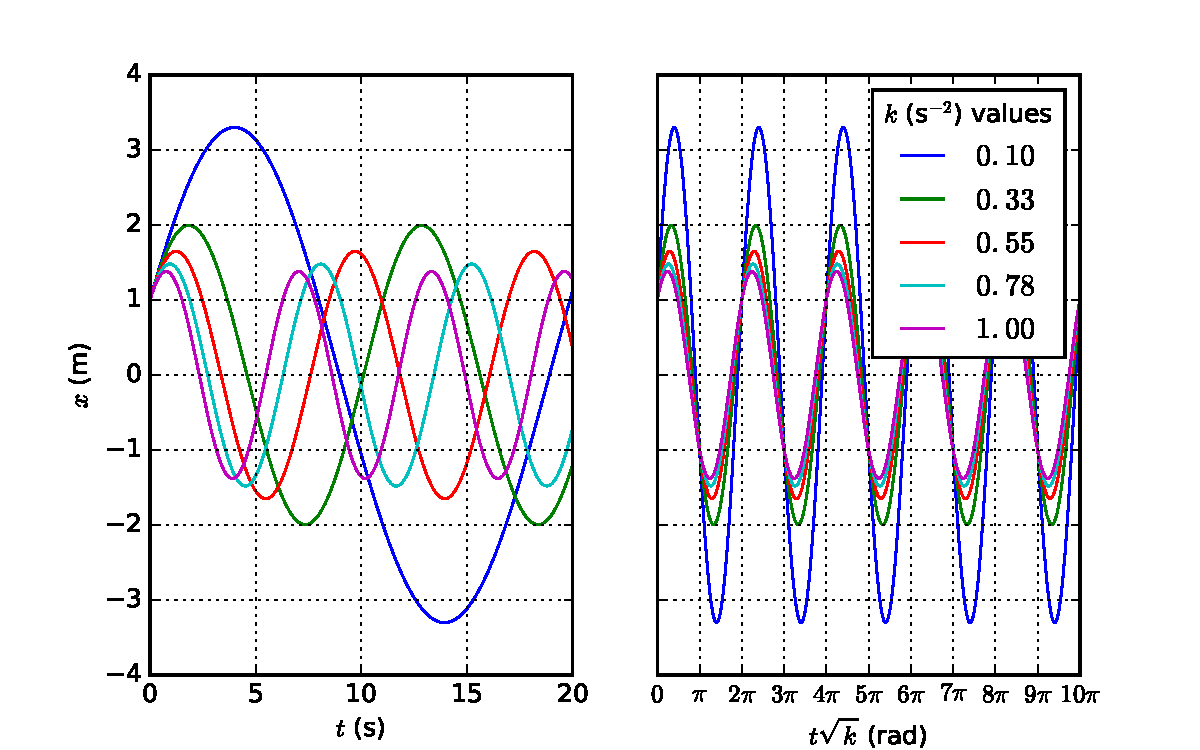
\includegraphics[width=0.9\linewidth]{plot.pdf}
\end{center}

\end{document}
              